\begin{figure}[p]
  \centering
  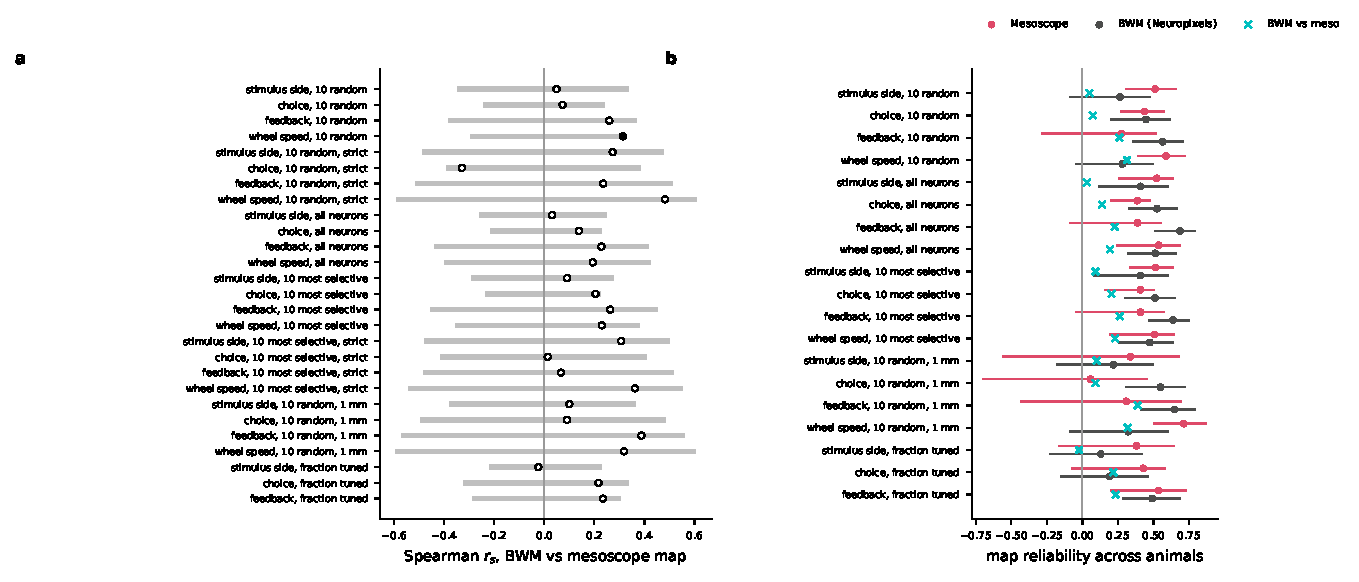
\includegraphics[width=7.00in,height=0.78\textheight,keepaspectratio]{si/si_spatial_null_panels.pdf}
  \caption{Are the bin-wise correlations between the modalities significant? Neighbouring bins are not independent (both maps are spatially smooth), so the naive $p$-values of the scatter plots are too small. 1 of 27 comparisons reach spatial $p<0.05$ (table in output/si\_spatial\_null.csv). \textbf{a} Spearman correlation between the BWM and the mesoscope map across the bins covered by both (dots; filled: spatial $p<0.05$), with the 95\,\% range of the spatial null (grey bars). Null: 1000 surrogate maps that keep the spatial autocorrelation (variogram) of the BWM map and 1000 of the mesoscope map (Burt et al. 2020: randomly permuted values smoothed over the $k$ nearest bins, $k$ and scale chosen to match the empirical variogram), each correlated with the other modality's map; the reported $p$ is the larger of the two. Rows: decoding from 10 random, all, or the 10 most selective neurons, with the original (0.4\,mm), strict or 1\,mm bins; fraction tuned. \textbf{b} Reliability of each modality's map across animals: animals split into two random halves (200 splits), per-bin maps of each half correlated over bins present in both (Spearman), Spearman--Brown corrected to the full data (median and 95\,\% range). Crosses: the BWM vs mesoscope correlation from a. A cross-modality correlation cannot be expected to exceed roughly the geometric mean of the two reliabilities.}
  \label{fig:si_spatial_null}
\end{figure}
